%%%%%%%%%%%%%%%%%%%
% RELATION EXTRACTION
%%%%%%%%%%%%%%%%%%%
\begin{frame}{Relation Extraction}
  \hh{Input}:  Sentences containing (\subj{entity}, \obj{slot value}). \\
  \hh{Output}: \rel{Relation} between \subj{entity} and \obj{slot value}.
\end{frame}


%%%%%%%%%%%%%%%%%%%
% DIST SUP
%%%%%%%%%%%%%%%%%%%
\begin{frame}{Distant Supervision}
\begin{center}
  
\includegraphics[height=0.5cm]{../img/freebase-logo.jpg} \hspace{0.5cm} (\subj{Barack Obama}, \rel{EmployedBy}, \obj{United States}) \\
  \vspace{0.5cm}
  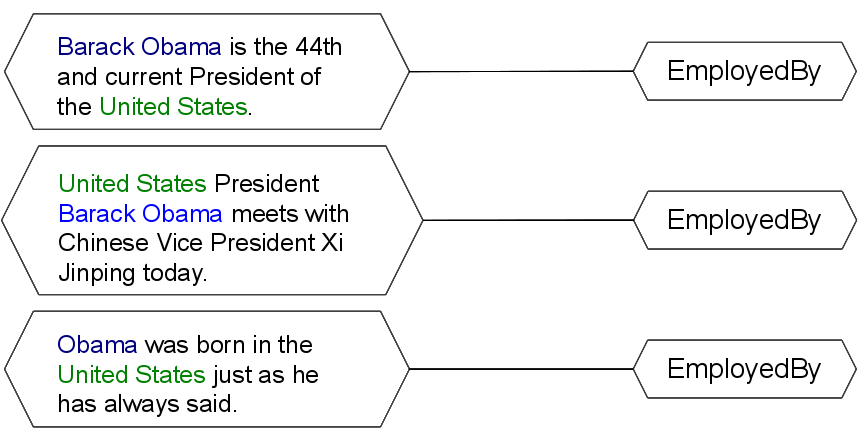
\includegraphics[height=5cm]{../img/distsup-naive.png}
\end{center}
\end{frame}

%%%%%%%%%%%%%%%%%%%
% MIML
%%%%%%%%%%%%%%%%%%%
\begin{frame}[noframenumbering]{Multiple-Instance Multiple-Label (MIML) Learning}
\begin{center}
  
\includegraphics[height=0.5cm]{../img/freebase-logo.jpg} \hspace{0.5cm} (\subj{Barack Obama}, \rel{EmployedBy}, \obj{United States}) \\
  \vspace{0.5cm}
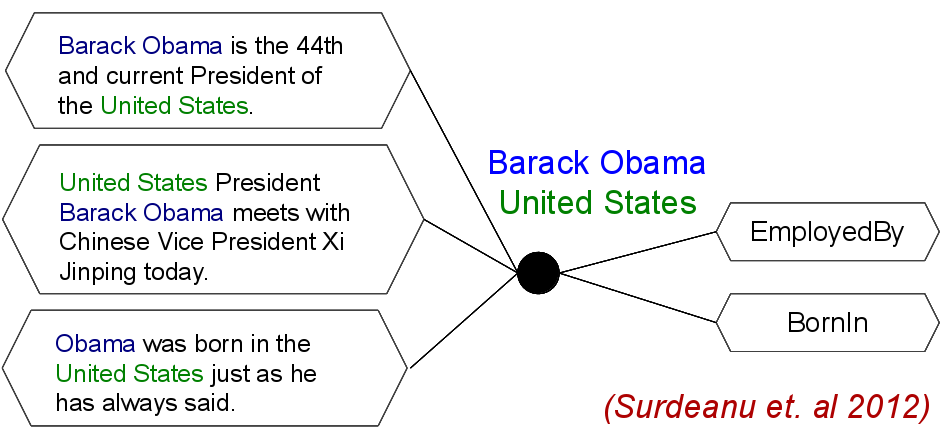
\includegraphics[height=5cm]{../img/distsup-miml.png}
\end{center}
\end{frame}

%%%%%%%%%%%%%%%%%%%
% MIML-RE
%%%%%%%%%%%%%%%%%%%
\def\title{MIML Relation Extraction (MIML-RE)}
\begin{frame}{Distant Supervision}
\begin{center}
  \dsPlate
  \hspace{0.5cm}
  \dsPlate
  \hspace{0.5cm}
  \dsPlate
\end{center}
\pause
\begin{textblock*}{6cm}(4.5cm,7.0cm)
  \textcolor<1-1>{white}{$\uparrow$ \w{\subj{\textcolor<1-1>{white}{Barack Obama}} is the 44th and current president of the \obj{\textcolor<1-1>{white}{United States}}}}
\end{textblock*}
\begin{textblock*}{6cm}(4.5cm,2.5cm)
  \textcolor<1-1>{white}{$\downarrow$ \rel{EmployedBy}}
\end{textblock*}
\end{frame}

\begin{frame}{Multiple-Instance}
\begin{center}
  \miPlate
\end{center}
\pause
\begin{textblock*}{4cm}(0.25cm,4.5cm)
  \textcolor<1-1>{white}{\textit{Latent} \\ per-mention relation $\rightarrow$}
\end{textblock*}
\end{frame}

\begin{frame}[noframenumbering]{Multiple-Instance Multiple-Label (MIML-RE)}
\begin{center}
  \mimlPlate
\end{center}
\end{frame}
